\documentclass[compress]{beamer}
%为了打印[]中还可加入handout或tran
%compress用于压缩侧边栏和上下两端的导航条,使文档紧凑
\usepackage{ctex}
%为支持汉字,由于ctex文档类中没有beamer的,故用普通文档类,再引入ctex包即可
%支持中文,其实该包会默认在document环境中加入CJK环境以支持中文,所以cjk包的
%命令它都支持
\usepackage{pgf,pgfarrows,pgfnodes,pgfautomata,pgfheaps}
%上面的包都是一些用pgf分布图的包
\usepackage{graphicx}%用于插入图片
\usepackage{beamerthemesplit}
\usepackage{multicol}
\usepackage{multirow}

%下面用于自定义模板

\beamertemplateshadingbackground{red!10}{structure!10}
%设置背景色由%10的红变为%10的结构颜色

\beamertemplatetransparentcoveredhigh
%隐藏文本高度透明

\beamertemplatetransparentcovereddynamicmedium
%使所有被隐藏的文本完全透明,动态

%\usetheme{Warsaw}
\usetheme{Singapore}
%\usetheme{Berkeley}
%\usetheme{Berlin}
%使用主题

\setbeamertemplate{footline}[page number]{}
%除掉页面下方的信息条
\setbeamertemplate{navigation symbols}{}
%除掉页面下方导航条

\begin{document}
\title{波形拟合反演震源机制的定权研究及误差评定}
\author{邓东平 2013202140004\\
	导师:朱良保教授}
\institute{
\includegraphics[height=3cm]{figures/whulogo.eps}\\
	武汉大学测绘学院}
\date{}
\AtBeginSection[]{
	\frame<handout:0>{
		\frametitle{预览}
		\tableofcontents[current,currentsubsection]
	}
}


\frame{\titlepage}
\transdissolve<5>
\section*{}
\frame{
\frametitle{概览}
\tableofcontents
}
\section{研究意义}
\frame{
	\frametitle{研究意义}
	\begin{itemize}
		\item 发震构造研究、灾害评估
		\item 区域应力、地震活动性
		\item 介质结构、海啸模拟等研究
	\end{itemize}
}
\section{研究现状和本文目标}
\subsection{研究现状}
\frame{
	\frametitle{研究现状}
	\begin{itemize}
		\item<+->{原理:}
			\begin{equation}
			\label{eq01}
			\left\{
			 \begin{array}{l}
			    U_z(r,\phi,0,\omega)=Z_{SS}{\cdot}s_2+Z_{DS}{\cdot}s_3+Z_{DD}{\cdot}s_1\\
			    U_r(r,\phi,0,\omega)=R_{SS}{\cdot}s_2+R_{DS}{\cdot}s_3+R_{DD}{\cdot}s_1\\
				U_{\phi}(r,\phi,0,\omega)=T_{SS}{\cdot}t_2+T_{DS}{\cdot}t_1\\
			 \end{array}
			\right.
			\end{equation}
		\item<+->{方法:}波形拟合(波形数据),格点搜索(公式\ref{eq01}非线性),
		\item<+->{应用:}CAP,CPS等代表性方法(程序)广泛应用
	\end{itemize}
}
\frame{
	\frametitle{研究现状}
	\begin{itemize}
		\item<+->{优点:}
			\begin{enumerate}[<+->]
			\item 波形数据充分应用了地震波信息
			\item 震源机制解空间较小,且正演合成迅速,格点搜索可快速反演
			\end{enumerate}
		\item<+->{问题:}
			\begin{enumerate}[<+->]
			\item 无法直接给出误差评价,无法有效识别病态问题
			\item CAP和CPS的加权方案不一致,数值相对大小冲突
			\end{enumerate}
	\end{itemize}
}
\subsection{本文目标}
\frame{
	\frametitle{\subsecname}
	\begin{itemize}
		\item 统一优化定权
		\item 针对CAP、CPS给出结果误差评价
	\end{itemize}
}

\section{解决方案}
\frame{
\frametitle{\subsecname}
	\begin{itemize}
		\item 优化定权
			\begin{enumerate}
			\item 分析二者定权的理论依据,联合定权解决差异
			\item 数值定量精化,结果尽量客观
			\end{enumerate}
		\item 针对CAP、CPS给出结果误差评价
			\begin{enumerate}
			\item 估计数据噪声
			\item 计算震源机制协方差矩阵
			\end{enumerate}
	\end{itemize}
}
\subsection{优化加权}
\frame{
\frametitle{优化加权}
	\begin{itemize}
		\item<+-> 联合加权
			\begin{enumerate}[<+->]
			\item CPS加权$W1$,考虑信噪比,权重随震中距单调递减
			\item CAP加权$W2$,考虑振幅调节,权重随震中距单调递增
			\item 信噪比和振幅调节均可提高数据质量,应联合统一$WT=W1*W2$
			\end{enumerate}
		\item<+-> 定量精化
			\begin{enumerate}[<+->]
			\item 利用震中距估计的$W1,W2$均较粗糙,改为由波形数据直接定量计算
			\item CAP加权估计$W2$的公式$(r/r_0)^p$中的参考参数$r_0,p$只能经验判定,主观性很强
			\end{enumerate}
		\item<+-> 本文最终权重
			\begin{enumerate}
			\item $WT=(1-NoiseStd/WaveStd)/L2norm$
			\end{enumerate}
	\end{itemize}
}
\subsection{误差估计}
\frame{
\frametitle{误差估计}
	\begin{columns}
	\column{0.4\textwidth}<1->
	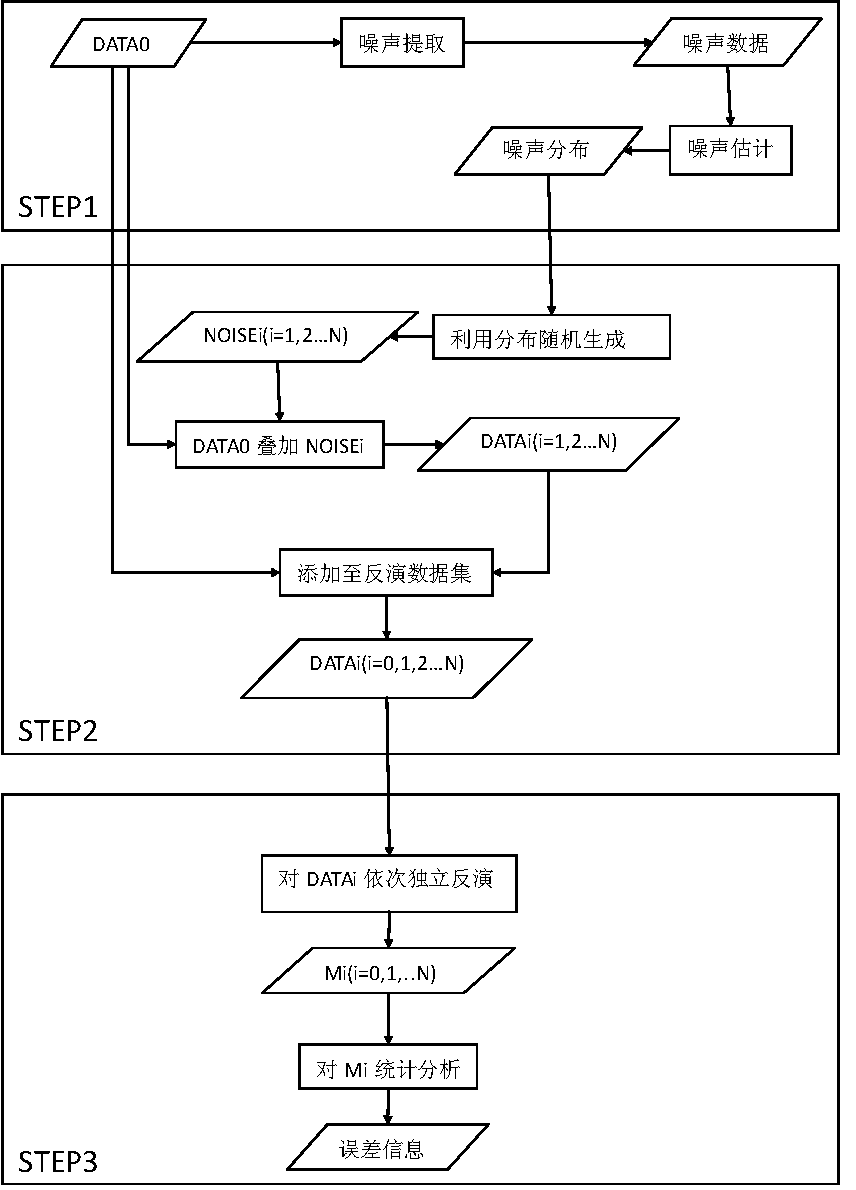
\includegraphics[height=7.5cm]{figures/flowchart.pdf}
	\column{0.6\textwidth}<1->
	\begin{itemize}
		\item<+-> STEP1 估计数据噪声
			\begin{enumerate}[<+->]
			\item 截取震前平静期数据样本
			\item 参数估计得到噪声分布函数(高斯)
			\end{enumerate}
		\item<+-> STEP2 随机生成模拟数据集
			\begin{enumerate}[<+->]
			\item 用噪声分布函数随机生成噪声数据
			\item 噪声数据与原始观测数据叠加,生成多组模拟观测数据
			\end{enumerate}
		\item<+-> STEP3 反演得解集并计算协方差矩阵
			\begin{enumerate}[<+->]
			\item 每组"观测"数据独立反演,得随机误差范围内解集
			\item 对解集统计分析,计算震源机制三参数协方差矩阵
			\end{enumerate}
	\end{itemize}
	\end{columns}
}
\section{实践检验}
\subsection{理论实验}
\frame{
	\frametitle{实验条件}
		走向250$^\circ$,倾角40$^\circ$,滑动角82$^\circ$,$M_w$震级6.5,震源深度17km 
		\begin{columns}
		\column{0.4\textwidth}<1->
		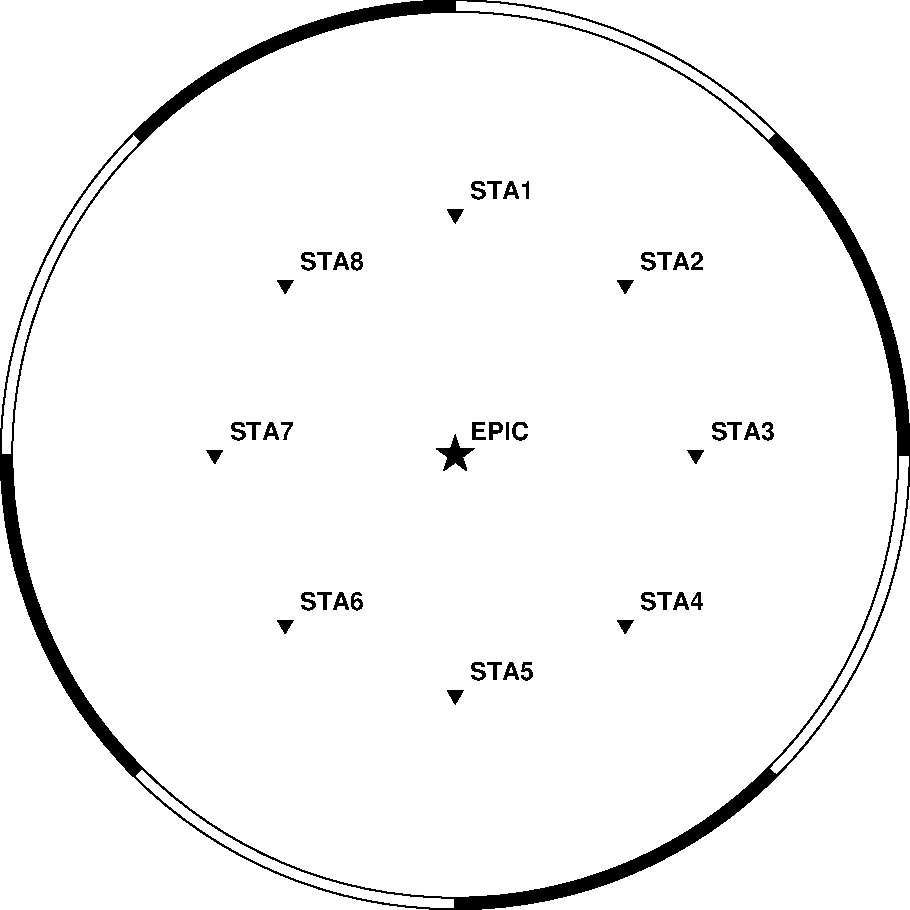
\includegraphics[height=3.5cm]{figures/fig3_01.pdf}
		\column{0.5\textwidth}<1->
		\centering
		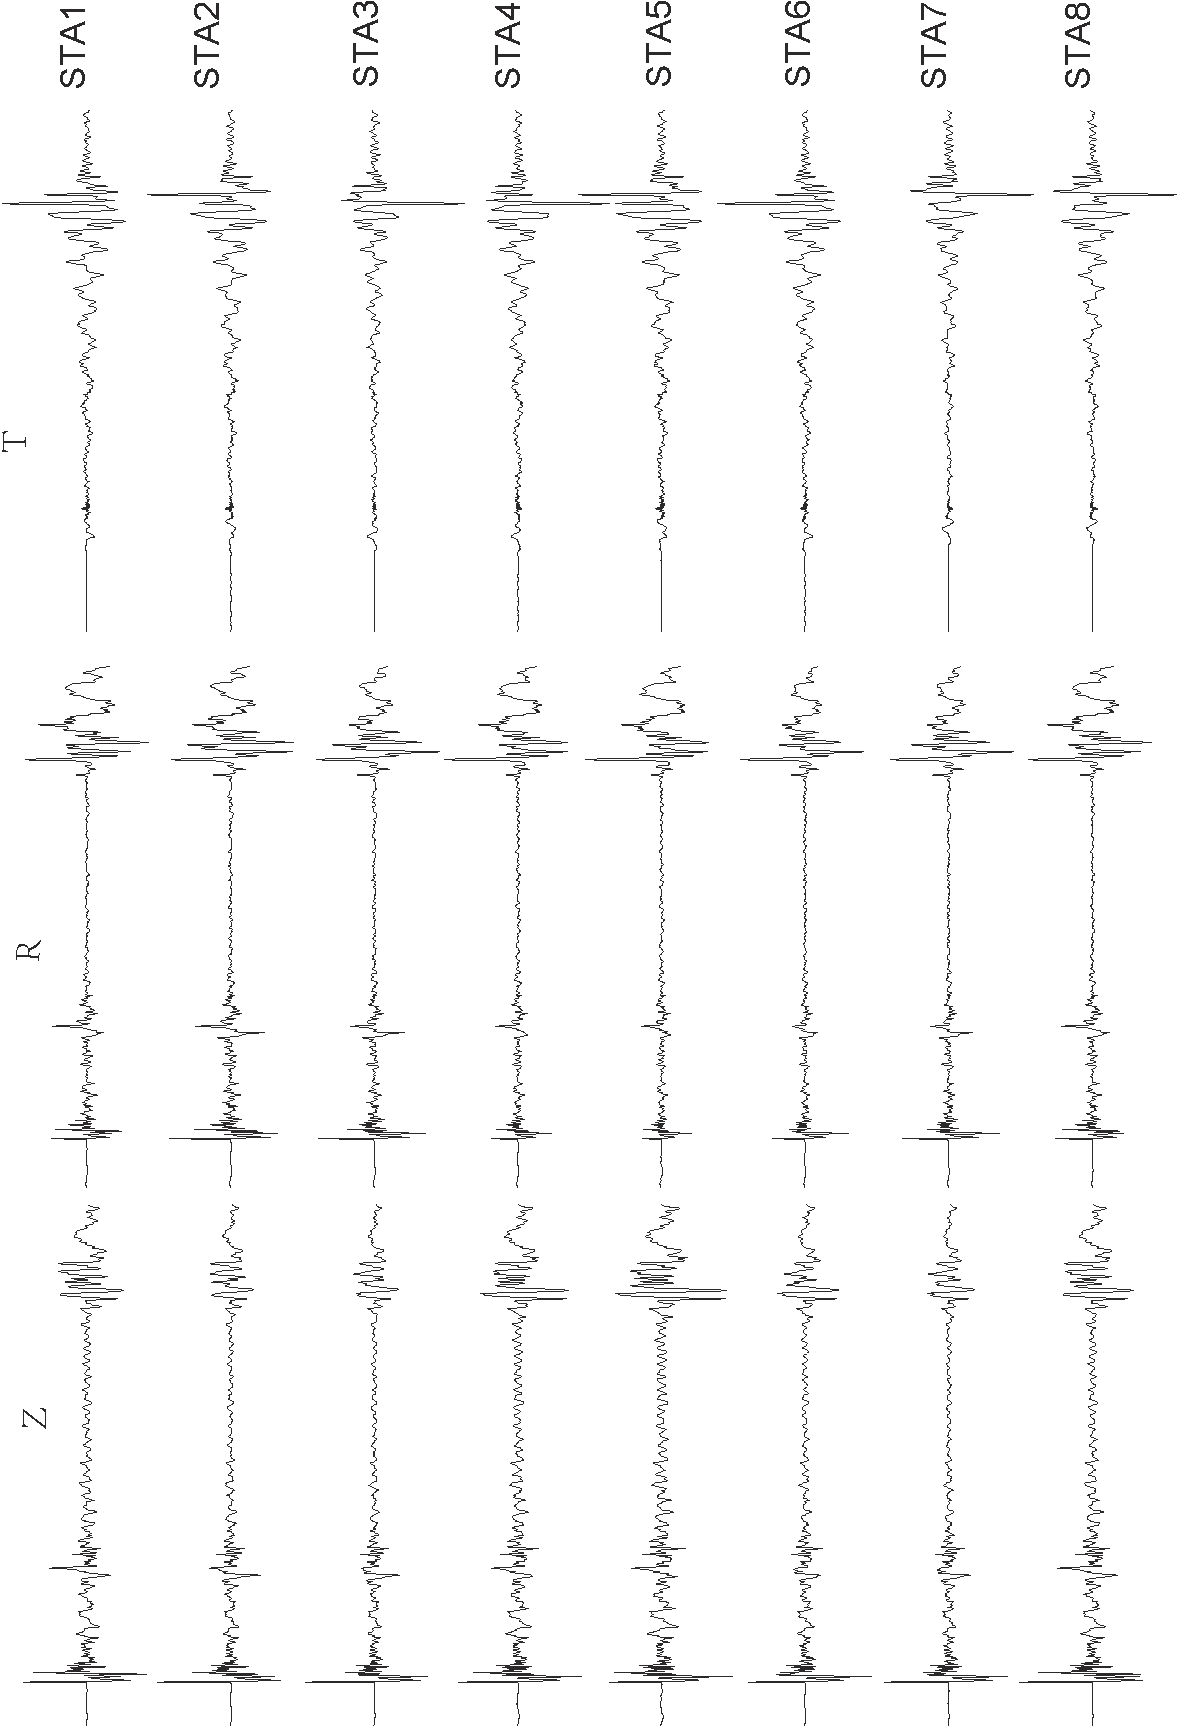
\includegraphics[height=5.5cm,angle=-90]{figures/fig3_02.pdf}
		\end{columns}
}
\frame{
	\frametitle{无噪实验}
	\begin{itemize}
		\item<+-> 数据拟合度100%,结果与理论设定一致
		\item<+-> 台站分布合理,满足反演要求
		\item<+-> 说明分辩核为单位矩阵
		\item<+-> 计算机数值计算引起的误差可忽略
	\end{itemize}
}
\frame{
	\frametitle{权重对比实验}
	\begin{table}[ht]
	\label{tab3_01}
    \begin{tabular}{c c c c c c c}
    \hline
     & 走向/$^\circ$ & 倾角/$^\circ$ & 滑动角/$^\circ$ & 深度/km & 拟合度 & 震级\\
    \hline
    真值	& 250 & 40 & 82 & 17 & 1	& 6.50\\
    W1		& 252 & 40 & 82 & 18 & 0.91 & 6.52\\
    W2		& 245 & 39 & 78 & 17 & 0.75 & 6.47\\
    WT		& 250 & 40 & 81 & 17 & 0.84 & 6.50\\
    \hline
    \end{tabular}
	\end{table}
	\begin{itemize}
		\item W1加权拟合度最高,但深度有偏差
		\item W2加权深度无偏差,拟合度最低
		\item 本文联合加权深度无偏,拟合度较高,综合效果最优
	\end{itemize}
}
\frame{
	\frametitle{噪声强度对比实验}
	\begin{table}[ht]
	\centering
	\label{tab3_06}
    \begin{tabular}{c c c c c}
    \hline
    加噪强度 & 走向/$^\circ$ & 倾角/$^\circ$ & 滑动角/$^\circ$ &拟合度 \\
    \hline
    无噪声		& 250 & 40 & 82  & 1\\
    低噪声($1.0\cdot10^{-6}$)		& 250$\pm$3 & 40$\pm$3 & 82$\pm$3 & 0.99 \\
    中等噪声($2.5\cdot10^{-6}$)	& 250$\pm$8 & 40$\pm$3 & 83$\pm$7 & 0.94 \\
    高噪声($5.0\cdot10^{-6}$)		& 246$\pm$18 & 40$\pm$6 & 78$\pm$17 & 0.87 \\
    超高噪声($1.0\cdot10^{-5}$)	& 245$\pm$30 & 42$\pm$14 & 84$\pm$36 & 0.65 \\
    \hline
    \end{tabular}
	\end{table}
	\begin{itemize}
		\item<+-> 局部线性近似下,理论误差大小与噪声强度成正比,与结果吻合
		\item<+-> 拟合度表征反演受噪声影响程度,结果表明拟合度低,误差大,稳定性差
		\item<+-> 各组反演结果均在误差范围内,证明了误差估计的准确性
	\end{itemize}
}
\subsection{实例应用}
\frame{
	\frametitle{芦山地震案例}
	\begin{columns}
	\column{0.4\textwidth}<1->
		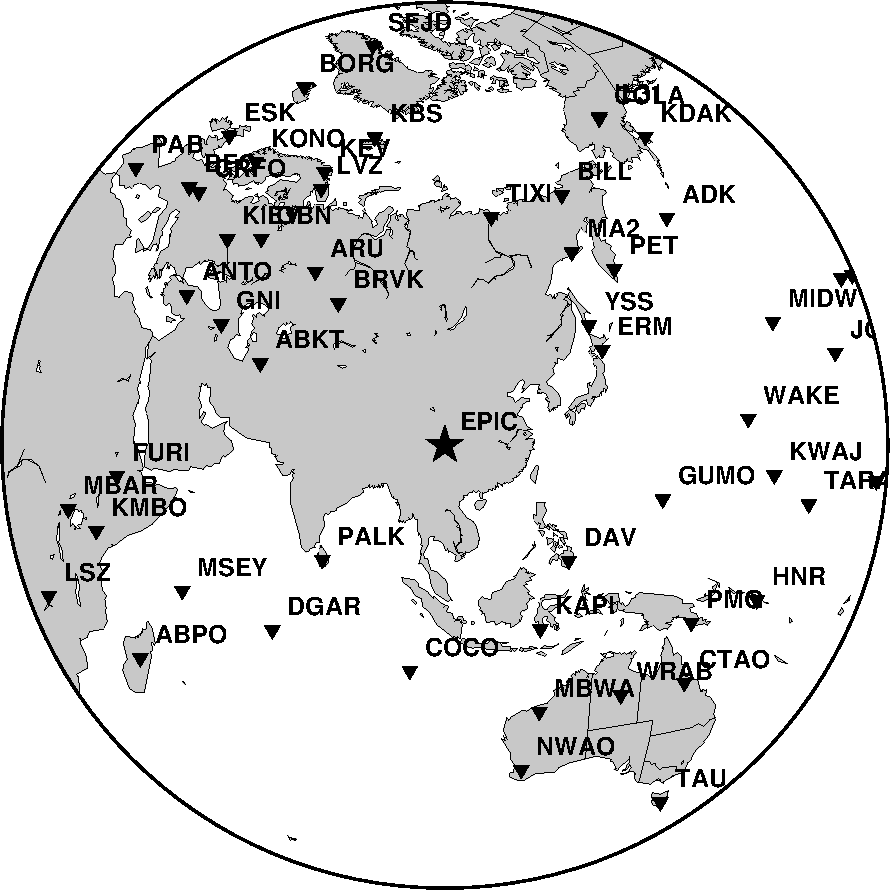
\includegraphics[height=5.0cm]{figures/fig4_02.pdf}
	\column{0.6\textwidth}<1->
	\begin{itemize}
		\item 远震P波和SH波联合反演
		\item 各道波形分别采用W1,W2以及本文的WT联合加权进行三次反演,对比择优
		\item 对最优结果进行误差评定
		\item 与他人成果对比
	\end{itemize}
	\end{columns}
}
\frame{
	\frametitle{权重对比分析——稳定性}
	\begin{columns}
	\column{0.4\textwidth}<1->
		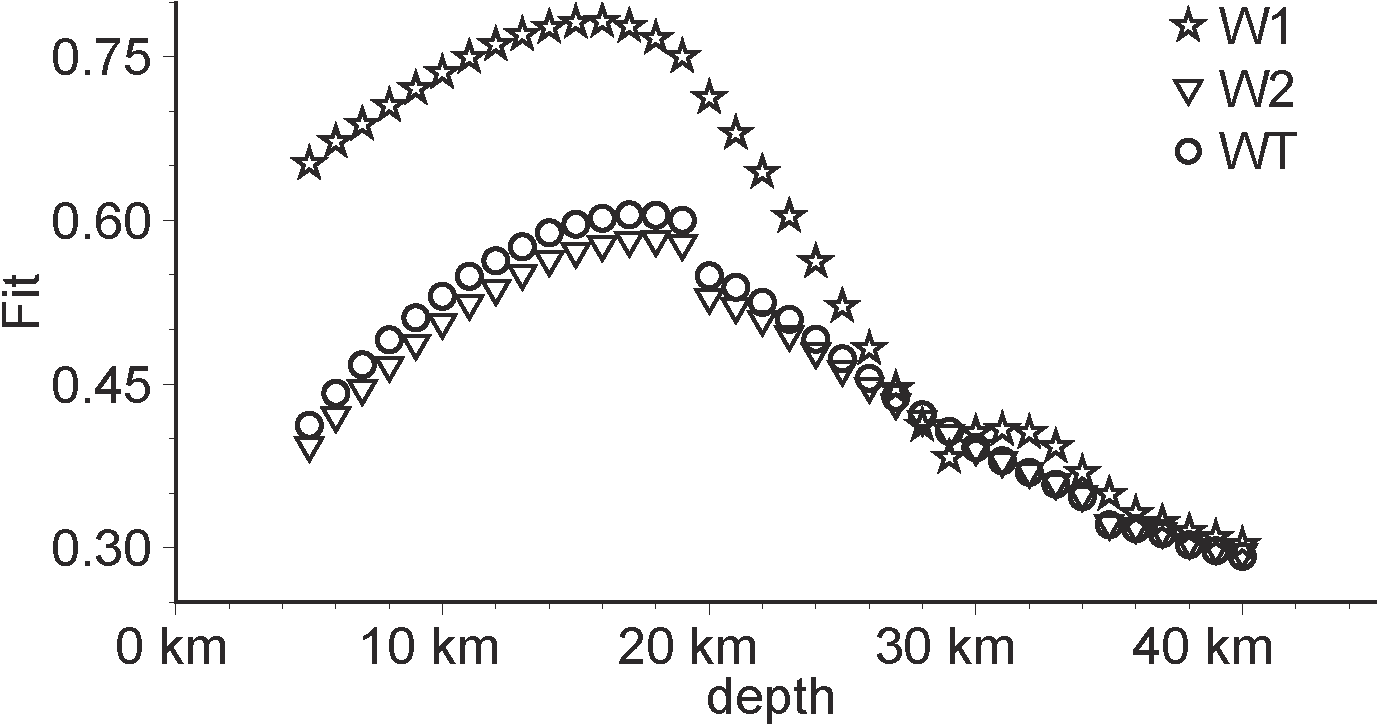
\includegraphics[height=3cm]{figures/fig4_03.pdf}
	\column{0.55\textwidth}<1->
	\begin{itemize}
		\item<+-> 拟合度W1>WT>W2,稳定性W1>WT>W2
		\item<+-> W1出现了双峰,深度约束不理想,易多解
	\end{itemize}
	\end{columns}
\begin{table}[ht]
\centering
\label{tab4_02}
    \begin{tabular}{c c c c}
    \hline
    加权方案 & 走向标准差/$^\circ$ & 倾角标准差/$^\circ$ & 滑动角标准差/$^\circ$\\
    \hline
    W1		&  1.03     &    0.00   & 0.61 \\
    W2		&  2.25     &    0.14   & 0.83 \\
    WT		&  1.66     &    0.00	& 0.59 \\
    \hline
    \end{tabular}
\end{table}
}
\frame{
	\frametitle{权重对比分析——可靠性}
	\begin{columns}
	\column{0.55\textwidth}<1->
		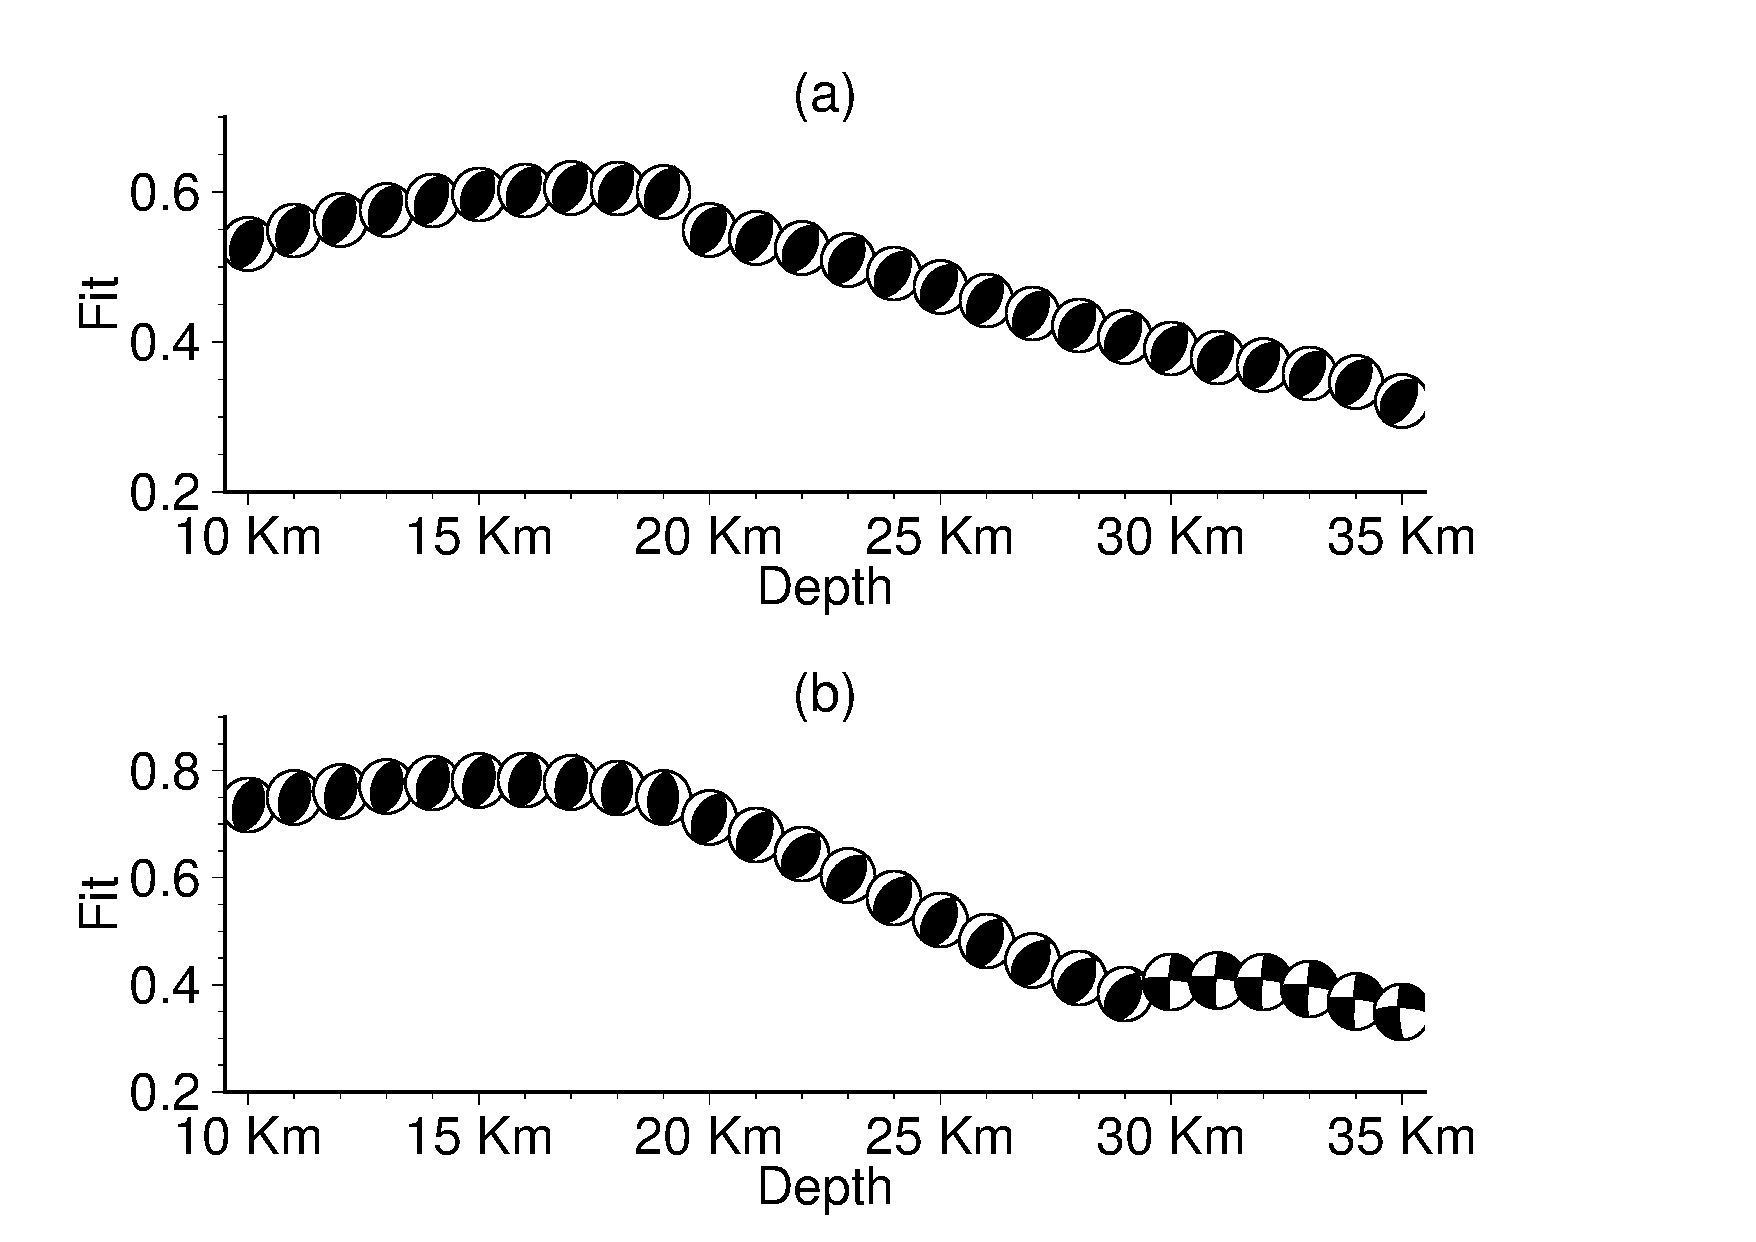
\includegraphics[height=5.0cm]{figures/fig4_04.pdf}
	\column{0.4\textwidth}<1->
	\begin{itemize}
		\item<+-> WT仅在18km左右出现极值,W1在18km,32km左右均有极值
		\item<+-> W1加权的震源机制随深度变化差异明显,易多解,不可靠
		\item<+-> 综合稳定性和可靠性考虑,WT加权最优
	\end{itemize}
	\end{columns}
}
\frame{
	\frametitle{WT加权误差评价}
		带误差的结果:走向$211^\circ\pm5^\circ$,倾角$41^\circ\pm1^\circ$,滑动角$94^\circ\pm2^\circ$
	\begin{columns}
	\column{0.55\textwidth}<1->
\begin{table}[ht]
\centering
\caption{震源机制各参数间相关性}
\label{tab4_03}
    \begin{tabular}{c c c c}
    \hline
    相关系数 & 走向 & 倾角 & 滑动角 \\
    \hline
	走向 		&1 			&0			&0.91\\
	倾角		&0			&1			&0\\
	滑动角		&0.91		&0			&1\\
    \hline
    \end{tabular}
\end{table}
	\column{0.4\textwidth}<1->
	\begin{itemize}
		\item<+-> 相关系数与理论实验较吻合,与预期一致
	\end{itemize}
	\end{columns}
}
\frame{
	\frametitle{他人成果对比}
\begin{table}[ht]
\centering
\label{tab4_04}
    \begin{tabular}{c c c c c c c c c c c }
    \hline
    研究者 & 美国地调局 & GCMT & 刘超 &韩立波等 &预测所 \\
    \hline
	深度/km			&12	&22	&15	&12	&15	\\
	走向/$^\circ$	&198&210&220&220&210\\ 
	倾角/$^\circ$	&33	&38	&35	&50	&47	\\
	滑动角/$^\circ$	&71	&96	&95	&107&90	\\
	$M_w$			&6.6&6.6&6.7&6.6&6.5\\
    \hline
    研究者 &  刘杰等 & 曾祥方等 & 谢祖军等 & 吕坚等 & 本文\\
    \hline
	深度/km			&19	&12	&16	&14	&17 \\
	走向/$^\circ$	&214&212&210&209&211\\ 
	倾角/$^\circ$	&39	&47	&44	&46	&41	\\
	滑动角/$^\circ$	&100&93	&91	&94	&94	\\
	$M_w$			&6.4&6.7&6.7&6.6&6.4\\
    \hline
    \end{tabular}
\end{table}
}
\frame{
	\frametitle{他人成果对比}
	\begin{columns}
	\column{0.55\textwidth}<1->
		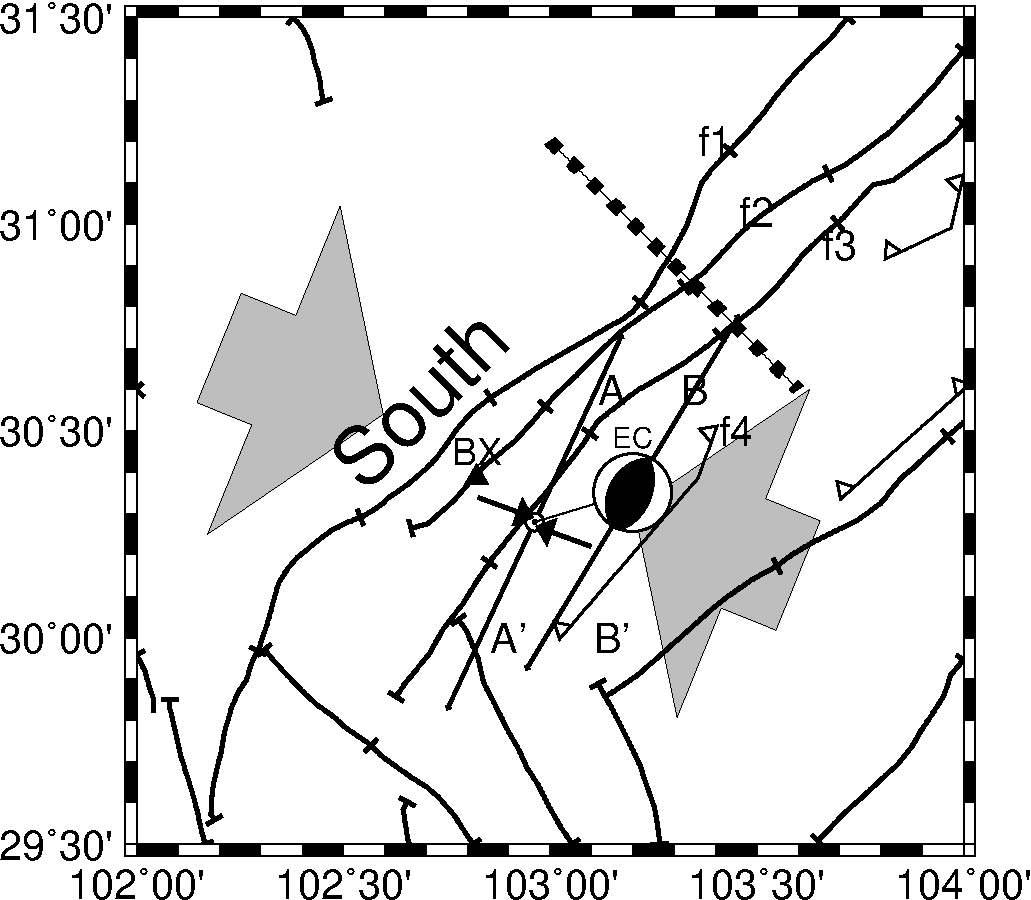
\includegraphics[height=5.0cm]{figures/fig4_06.pdf}
	\column{0.4\textwidth}<1->
	\begin{itemize}
		\item<+-> 震源机制显示的主应力与灰色箭头代表的区域主应力方向以及应力实测(BX)一致
		\item<+-> 与剪切波快轴暗示的主应力方向一致,且走向和双差重定位的余震空间分布吻合
		\item<+-> 与龙门山断裂带南段的走向和构造运动背景吻合
	\end{itemize}
	\end{columns}
}
\section{总结和展望}
\frame{
	\frametitle{工作总结}
	\begin{itemize}
		\item<+-> 核心工作,提出了一种误差评估方案解决CAP、CPS误差缺失的问题,并从理论和实践分别进行论证方法的有效性
		\item<+-> 在CAP和CPS基础上针对其加权"冲突",提出一联合加权的统一方案,并定量精化,优化加权
		\item<+-> 芦山地震的震源机制反演表明,发震原因是由区域水平西北-东南向的挤压应力长期积累导致的高倾角逆冲位错
	\end{itemize}
}
\frame{
	\frametitle{不足和展望}
	\begin{itemize}
		\item<+-> 目前的误差评价方案仅能分析随机噪声的影响,对模型偏差等系统性误差无能为力
		\item<+-> 该误差分析方法要求大量样本统计,震要重复反演,大大增加了计算量
		\item<+-> 目标:应更系统全面地分析各种误差及适当减少计算量
	\end{itemize}
}
\frame{
	\frametitle{结束}
		感谢您的宝贵时间
}
\end{document}
